\documentclass{standalone}
\usepackage{tikz}
\usetikzlibrary{patterns, positioning}
\usepackage[sfdefault]{ClearSans} %% option 'sfdefault' activates Clear Sans as the default text font
\usepackage[T1]{fontenc}

\begin{document}
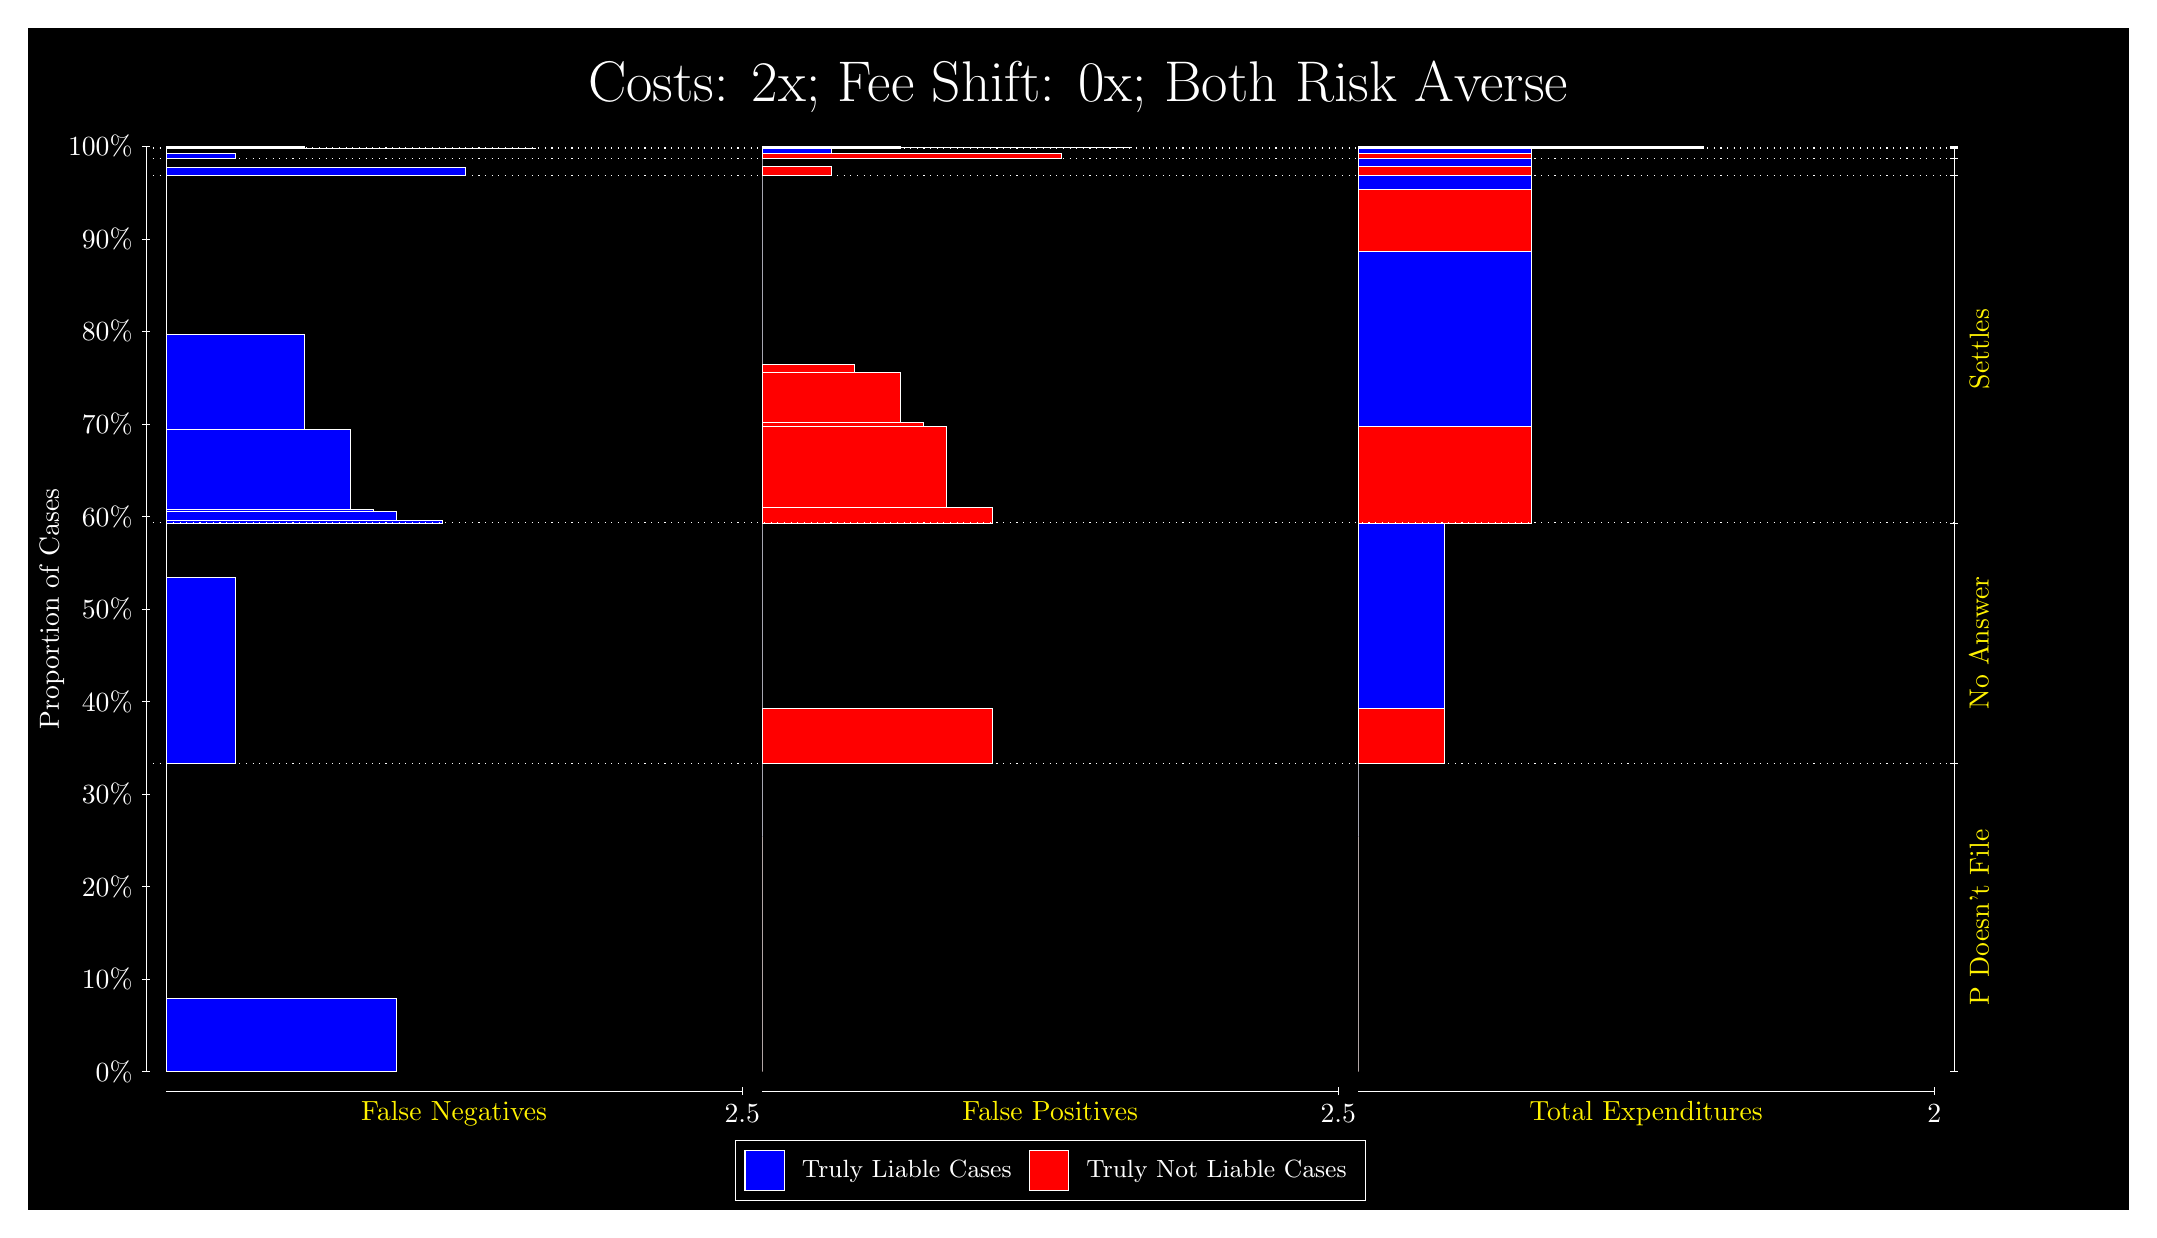
\begin{tikzpicture}
\draw[fill=black] (0,0) rectangle (26.667,15);
\draw[text=white] (0,13.5) rectangle (26.667,15) node[midway] {\huge Costs: 2x; Fee Shift: 0x; Both Risk Averse};
\draw[white, very thin] (1.5,1.75) -- (1.5,13.5);
\node[rotate=90, text=white, anchor=center] at (0.3, 7.625) {Proportion of Cases};
\draw[white, very thin] (1.45,1.75) -- (1.55,1.75);
\node[text=white, anchor=east] at (1.45, 1.75) {0\%};
\draw[white, very thin] (1.45,2.925) -- (1.55,2.925);
\node[text=white, anchor=east] at (1.45, 2.925) {10\%};
\draw[white, very thin] (1.45,4.1) -- (1.55,4.1);
\node[text=white, anchor=east] at (1.45, 4.1) {20\%};
\draw[white, very thin] (1.45,5.275) -- (1.55,5.275);
\node[text=white, anchor=east] at (1.45, 5.275) {30\%};
\draw[white, very thin] (1.45,6.45) -- (1.55,6.45);
\node[text=white, anchor=east] at (1.45, 6.45) {40\%};
\draw[white, very thin] (1.45,7.625) -- (1.55,7.625);
\node[text=white, anchor=east] at (1.45, 7.625) {50\%};
\draw[white, very thin] (1.45,8.8) -- (1.55,8.8);
\node[text=white, anchor=east] at (1.45, 8.8) {60\%};
\draw[white, very thin] (1.45,9.975) -- (1.55,9.975);
\node[text=white, anchor=east] at (1.45, 9.975) {70\%};
\draw[white, very thin] (1.45,11.15) -- (1.55,11.15);
\node[text=white, anchor=east] at (1.45, 11.15) {80\%};
\draw[white, very thin] (1.45,12.325) -- (1.55,12.325);
\node[text=white, anchor=east] at (1.45, 12.325) {90\%};
\draw[white, very thin] (1.45,13.5) -- (1.55,13.5);
\node[text=white, anchor=east] at (1.45, 13.5) {100\%};

\draw[white, very thin] (24.457,1.75) -- (24.457,13.5);
\draw[white, very thin] (24.407,1.75) -- (24.507,1.75);
\node[anchor=west] at (24.407, 1.75) {};
\draw[white, very thin] (24.407,5.6667) -- (24.507,5.6667);
\node[anchor=west] at (24.407, 5.6667) {};
\draw[white, very thin] (24.407,8.7187) -- (24.507,8.7187);
\node[anchor=west] at (24.407, 8.7187) {};
\draw[white, very thin] (24.407,13.13) -- (24.507,13.13);
\node[anchor=west] at (24.407, 13.13) {};
\draw[white, very thin] (24.407,13.349) -- (24.507,13.349);
\node[anchor=west] at (24.407, 13.349) {};
\draw[white, very thin] (24.407,13.474) -- (24.507,13.474);
\node[anchor=west] at (24.407, 13.474) {};
\draw[white, very thin] (24.407,13.486) -- (24.507,13.486);
\node[anchor=west] at (24.407, 13.486) {};
\draw[white, very thin] (24.407,13.5) -- (24.507,13.5);
\node[anchor=west] at (24.407, 13.5) {};

\draw[white, very thin, fill=blue] (1.75,1.75) rectangle (4.6775,2.685);
\draw[white, very thin, fill=red] (1.75,2.685) rectangle (1.75,5.6667);
\draw[white, very thin, fill=blue] (1.75,5.6667) rectangle (2.6283,8.0243);
\draw[white, very thin, fill=red] (1.75,8.0243) rectangle (1.75,8.7187);
\draw[white, very thin, fill=blue] (1.75,8.7187) rectangle (5.2631,8.7461);
\draw[white, very thin, fill=blue] (1.75,8.7461) rectangle (4.6775,8.8655);
\draw[white, very thin, fill=blue] (1.75,8.8655) rectangle (4.3848,8.8907);
\draw[white, very thin, fill=blue] (1.75,8.8907) rectangle (4.092,9.9122);
\draw[white, very thin, fill=blue] (1.75,9.9122) rectangle (3.5065,11.113);
\draw[white, very thin, fill=red] (1.75,11.113) rectangle (1.75,13.13);
\draw[white, very thin, fill=blue] (1.75,13.13) rectangle (5.5558,13.237);
\draw[white, very thin, fill=red] (1.75,13.237) rectangle (1.75,13.349);
\draw[white, very thin, fill=blue] (1.75,13.349) rectangle (2.6283,13.416);
\draw[white, very thin, fill=red] (1.75,13.416) rectangle (1.75,13.474);
\draw[white, very thin, fill=blue] (1.75,13.474) rectangle (6.4341,13.478);
\draw[white, very thin, fill=red] (1.75,13.478) rectangle (1.75,13.486);
\draw[white, very thin, fill=blue] (1.75,13.486) rectangle (3.5065,13.496);
\draw[white, very thin, fill=red] (1.75,13.496) rectangle (1.75,13.5);
\draw[white, very thin, fill=red] (9.3189,1.75) rectangle (9.3189,4.7317);
\draw[white, very thin, fill=blue] (9.3189,4.7317) rectangle (9.3189,5.6667);
\draw[white, very thin, fill=red] (9.3189,5.6667) rectangle (12.246,6.3611);
\draw[white, very thin, fill=blue] (9.3189,6.3611) rectangle (9.3189,8.7187);
\draw[white, very thin, fill=red] (9.3189,8.7187) rectangle (12.246,8.9146);
\draw[white, very thin, fill=red] (9.3189,8.9146) rectangle (11.661,9.9397);
\draw[white, very thin, fill=red] (9.3189,9.9397) rectangle (11.368,9.9896);
\draw[white, very thin, fill=red] (9.3189,9.9896) rectangle (11.075,10.636);
\draw[white, very thin, fill=red] (9.3189,10.636) rectangle (10.49,10.736);
\draw[white, very thin, fill=blue] (9.3189,10.736) rectangle (9.3189,13.13);
\draw[white, very thin, fill=red] (9.3189,13.13) rectangle (10.197,13.243);
\draw[white, very thin, fill=blue] (9.3189,13.243) rectangle (9.3189,13.349);
\draw[white, very thin, fill=red] (9.3189,13.349) rectangle (13.125,13.407);
\draw[white, very thin, fill=blue] (9.3189,13.407) rectangle (10.197,13.474);
\draw[white, very thin, fill=red] (9.3189,13.474) rectangle (11.075,13.481);
\draw[white, very thin, fill=blue] (9.3189,13.481) rectangle (9.3189,13.486);
\draw[white, very thin, fill=red] (9.3189,13.486) rectangle (14.003,13.49);
\draw[white, very thin, fill=blue] (9.3189,13.49) rectangle (11.075,13.5);
\draw[white, very thin, fill=red] (16.888,1.75) rectangle (16.888,4.7317);
\draw[white, very thin, fill=blue] (16.888,4.7317) rectangle (16.888,5.6667);
\draw[white, very thin, fill=red] (16.888,5.6667) rectangle (17.986,6.3611);
\draw[white, very thin, fill=blue] (16.888,6.3611) rectangle (17.986,8.7187);
\draw[white, very thin, fill=red] (16.888,8.7187) rectangle (19.083,9.9397);
\draw[white, very thin, fill=blue] (16.888,9.9397) rectangle (19.083,12.162);
\draw[white, very thin, fill=red] (16.888,12.162) rectangle (19.083,12.958);
\draw[white, very thin, fill=blue] (16.888,12.958) rectangle (19.083,13.13);
\draw[white, very thin, fill=red] (16.888,13.13) rectangle (19.083,13.243);
\draw[white, very thin, fill=blue] (16.888,13.243) rectangle (19.083,13.349);
\draw[white, very thin, fill=red] (16.888,13.349) rectangle (19.083,13.407);
\draw[white, very thin, fill=blue] (16.888,13.407) rectangle (19.083,13.474);
\draw[white, very thin, fill=red] (16.888,13.474) rectangle (21.279,13.481);
\draw[white, very thin, fill=blue] (16.888,13.481) rectangle (21.279,13.486);
\draw[white, very thin, fill=red] (16.888,13.486) rectangle (21.279,13.49);
\draw[white, very thin, fill=blue] (16.888,13.49) rectangle (21.279,13.5);
\draw[white, dotted] (1.5,5.6667) -- (24.457,5.6667);
\draw[white, dotted] (1.5,8.7187) -- (24.457,8.7187);
\draw[white, dotted] (1.5,13.13) -- (24.457,13.13);
\draw[white, dotted] (1.5,13.349) -- (24.457,13.349);
\draw[white, dotted] (1.5,13.474) -- (24.457,13.474);
\draw[white, dotted] (1.5,13.486) -- (24.457,13.486);
\draw[white, very thin] (1.75,1.5) -- (9.0689,1.5);
\node[text=yellow, anchor=north] at (5.4094, 1.5) {False Negatives};
\draw[white, very thin] (9.0689,1.45) -- (9.0689,1.55);
\node[text=white, anchor=north] at (9.0689, 1.45) {2.5};

\draw[white, very thin] (9.3189,1.5) -- (16.638,1.5);
\node[text=yellow, anchor=north] at (12.978, 1.5) {False Positives};
\draw[white, very thin] (16.638,1.45) -- (16.638,1.55);
\node[text=white, anchor=north] at (16.638, 1.45) {2.5};

\draw[white, very thin] (16.888,1.5) -- (24.207,1.5);
\node[text=yellow, anchor=north] at (20.547, 1.5) {Total Expenditures};
\draw[white, very thin] (24.207,1.45) -- (24.207,1.55);
\node[text=white, anchor=north] at (24.207, 1.45) {2};

\node[text=yellow, centered, rotate=90] at (24.777, 3.7084) {P Doesn't File};
\node[text=yellow, centered, rotate=90] at (24.777, 7.1927) {No Answer};
\node[text=yellow, centered, rotate=90] at (24.777, 10.925) {Settles};





\draw (12.978300999999998,1.5) node[draw=none] (baseCoordinate) {};
\begin{scope}[align=center]
        \matrix[scale=0.5, draw=white, below=0.5cm of baseCoordinate, nodes={draw}, column sep=0.1cm]{
            \node[rectangle, draw, minimum width=0.5cm, minimum height=0.5cm, fill=blue] {}; &
            \node[draw=none, font=\small, text=white] (B) {Truly Liable Cases}; &
            \node[rectangle, draw, minimum width=0.5cm, minimum height=0.5cm, fill=red] {}; &
            \node[draw=none, font=\small, text=white] (B) {Truly Not Liable Cases}; \\
            };
\end{scope}

\end{tikzpicture}
\end{document}